% Options for packages loaded elsewhere
\PassOptionsToPackage{unicode}{hyperref}
\PassOptionsToPackage{hyphens}{url}
%
\documentclass[
  14pt,
  ignorenonframetext,
  aspectratio=169,
]{beamer}
\usepackage{pgfpages}
\setbeamertemplate{caption}[numbered]
\setbeamertemplate{caption label separator}{: }
\setbeamercolor{caption name}{fg=normal text.fg}
\beamertemplatenavigationsymbolsempty
% Prevent slide breaks in the middle of a paragraph
\widowpenalties 1 10000
\raggedbottom

\usepackage{amsmath,amssymb}
\usepackage{iftex}
\ifPDFTeX
  \usepackage[T1]{fontenc}
  \usepackage[utf8]{inputenc}
  \usepackage{textcomp} % provide euro and other symbols
\else % if luatex or xetex
  \usepackage{unicode-math}
  \defaultfontfeatures{Scale=MatchLowercase}
  \defaultfontfeatures[\rmfamily]{Ligatures=TeX,Scale=1}
\fi
\usepackage{lmodern}
\usetheme[]{monash}
\ifPDFTeX\else  
    % xetex/luatex font selection
\fi
% Use upquote if available, for straight quotes in verbatim environments
\IfFileExists{upquote.sty}{\usepackage{upquote}}{}
\IfFileExists{microtype.sty}{% use microtype if available
  \usepackage[]{microtype}
  \UseMicrotypeSet[protrusion]{basicmath} % disable protrusion for tt fonts
}{}
\makeatletter
\@ifundefined{KOMAClassName}{% if non-KOMA class
  \IfFileExists{parskip.sty}{%
    \usepackage{parskip}
  }{% else
    \setlength{\parindent}{0pt}
    \setlength{\parskip}{6pt plus 2pt minus 1pt}}
}{% if KOMA class
  \KOMAoptions{parskip=half}}
\makeatother
\usepackage{xcolor}
\newif\ifbibliography
\setlength{\emergencystretch}{3em} % prevent overfull lines
\setcounter{secnumdepth}{-\maxdimen} % remove section numbering

\usepackage{color}
\usepackage{fancyvrb}
\newcommand{\VerbBar}{|}
\newcommand{\VERB}{\Verb[commandchars=\\\{\}]}
\DefineVerbatimEnvironment{Highlighting}{Verbatim}{commandchars=\\\{\}}
% Add ',fontsize=\small' for more characters per line
\usepackage{framed}
\definecolor{shadecolor}{RGB}{248,248,248}
\newenvironment{Shaded}{\begin{snugshade}}{\end{snugshade}}
\newcommand{\AlertTok}[1]{\textcolor[rgb]{0.94,0.16,0.16}{#1}}
\newcommand{\AnnotationTok}[1]{\textcolor[rgb]{0.56,0.35,0.01}{\textbf{\textit{#1}}}}
\newcommand{\AttributeTok}[1]{\textcolor[rgb]{0.77,0.63,0.00}{#1}}
\newcommand{\BaseNTok}[1]{\textcolor[rgb]{0.00,0.00,0.81}{#1}}
\newcommand{\BuiltInTok}[1]{\textcolor[rgb]{0.00,0.00,0.00}{#1}}
\newcommand{\CharTok}[1]{\textcolor[rgb]{0.31,0.60,0.02}{#1}}
\newcommand{\CommentTok}[1]{\textcolor[rgb]{0.56,0.35,0.01}{\textit{#1}}}
\newcommand{\CommentVarTok}[1]{\textcolor[rgb]{0.56,0.35,0.01}{\textbf{\textit{#1}}}}
\newcommand{\ConstantTok}[1]{\textcolor[rgb]{0.00,0.00,0.00}{#1}}
\newcommand{\ControlFlowTok}[1]{\textcolor[rgb]{0.13,0.29,0.53}{\textbf{#1}}}
\newcommand{\DataTypeTok}[1]{\textcolor[rgb]{0.13,0.29,0.53}{#1}}
\newcommand{\DecValTok}[1]{\textcolor[rgb]{0.00,0.00,0.81}{#1}}
\newcommand{\DocumentationTok}[1]{\textcolor[rgb]{0.56,0.35,0.01}{\textbf{\textit{#1}}}}
\newcommand{\ErrorTok}[1]{\textcolor[rgb]{0.64,0.00,0.00}{\textbf{#1}}}
\newcommand{\ExtensionTok}[1]{\textcolor[rgb]{0.00,0.00,0.00}{#1}}
\newcommand{\FloatTok}[1]{\textcolor[rgb]{0.00,0.00,0.81}{#1}}
\newcommand{\FunctionTok}[1]{\textcolor[rgb]{0.00,0.00,0.00}{#1}}
\newcommand{\ImportTok}[1]{\textcolor[rgb]{0.00,0.00,0.00}{#1}}
\newcommand{\InformationTok}[1]{\textcolor[rgb]{0.56,0.35,0.01}{\textbf{\textit{#1}}}}
\newcommand{\KeywordTok}[1]{\textcolor[rgb]{0.13,0.29,0.53}{\textbf{#1}}}
\newcommand{\NormalTok}[1]{\textcolor[rgb]{0.00,0.00,0.00}{#1}}
\newcommand{\OperatorTok}[1]{\textcolor[rgb]{0.81,0.36,0.00}{\textbf{#1}}}
\newcommand{\OtherTok}[1]{\textcolor[rgb]{0.56,0.35,0.01}{#1}}
\newcommand{\PreprocessorTok}[1]{\textcolor[rgb]{0.56,0.35,0.01}{\textit{#1}}}
\newcommand{\RegionMarkerTok}[1]{\textcolor[rgb]{0.00,0.00,0.00}{#1}}
\newcommand{\SpecialCharTok}[1]{\textcolor[rgb]{0.00,0.00,0.00}{#1}}
\newcommand{\SpecialStringTok}[1]{\textcolor[rgb]{0.31,0.60,0.02}{#1}}
\newcommand{\StringTok}[1]{\textcolor[rgb]{0.31,0.60,0.02}{#1}}
\newcommand{\VariableTok}[1]{\textcolor[rgb]{0.00,0.00,0.00}{#1}}
\newcommand{\VerbatimStringTok}[1]{\textcolor[rgb]{0.31,0.60,0.02}{#1}}
\newcommand{\WarningTok}[1]{\textcolor[rgb]{0.56,0.35,0.01}{\textbf{\textit{#1}}}}

\providecommand{\tightlist}{%
  \setlength{\itemsep}{0pt}\setlength{\parskip}{0pt}}\usepackage{longtable,booktabs,array}
\usepackage{calc} % for calculating minipage widths
\usepackage{caption}
% Make caption package work with longtable
\makeatletter
\def\fnum@table{\tablename~\thetable}
\makeatother
\usepackage{graphicx}
\makeatletter
\def\maxwidth{\ifdim\Gin@nat@width>\linewidth\linewidth\else\Gin@nat@width\fi}
\def\maxheight{\ifdim\Gin@nat@height>\textheight\textheight\else\Gin@nat@height\fi}
\makeatother
% Scale images if necessary, so that they will not overflow the page
% margins by default, and it is still possible to overwrite the defaults
% using explicit options in \includegraphics[width, height, ...]{}
\setkeys{Gin}{width=\maxwidth,height=\maxheight,keepaspectratio}
% Set default figure placement to htbp
\makeatletter
\def\fps@figure{htbp}
\makeatother

% Colors
\definecolor{shadecolor}{RGB}{225,225,225}
\setbeamercolor{description item}{fg=Orange}
\definecolor{MonashBlue}{RGB}{66,109,152}
\definecolor{burntorange}{rgb}{0.8, 0.33, 0.0}

% Packages
\usepackage{amsmath, bm, amssymb, amsthm, mathrsfs,pifont}
\usepackage{url}
\usepackage{multirow, booktabs, float, textcmds, siunitx}
\usepackage{bm,booktabs,animate,ragged2e,multicol,microtype,hyperref}
\usepackage{fontawesome5}

% Figures
\graphicspath{{figs/}}

% Fonts
\fontsize{13}{15}\sf
\setbeamerfont{title}{series=\bfseries,parent=structure,size=\fontsize{24}{24}}
\ifcsname Shaded\endcsname
  \definecolor{shadecolor}{RGB}{225,225,225}
  \renewenvironment{Shaded}{\vspace*{0.15cm}\color{black}\fontsize{10}{10}\sf\begin{snugshade}\color{black}}{\end{snugshade}}
\fi

% gt dependencies
\usepackage{longtable,caption,setspace}
\captionsetup{font={small,stretch=0.80}}

% My definitions

\def\E{\text{E}}
\def\V{\text{Var}}
\def\up#1{\raisebox{-0.3cm}{#1}}
\def\pred#1#2#3{\hat{#1}_{#2|#3}}
\def\damped{$_\text{d}$}
\def\h+{h_{m}^{+}}
\def\str#1{\rlap{#1}\textcolor{red}{\rule{1cm}{0.1cm}}}

\def\st#1{\rlap{#1}\textcolor{red}{\rule{1cm}{0.1cm}}}
\def\bY{\bm{y}}
\def\by{\bm{y}}
\def\bS{\bm{S}}
\def\bI{\text{\rm\textbf{I}}}
\def\bbeta{\bm{\beta}}
\def\bSigma{\bm{\Sigma}}
\def\bW{\bm{\Sigma}}
\def\Var{\text{Var}}
\def\var{\text{Var}}
\def\bOmega{\bm{\Omega}}
\def\bLambda{\bm{\Lambda}}
\let\mc\multicolumn
\def\hl{\color[RGB]{230, 172, 0}}

\def\forecast{\begin{alertblock}{}\fontsize{10}{11}\sf
 A forecast is an estimate of the probability distribution of a variable to be observed in the future.
\end{alertblock}}

\def\simfutures{\begin{textblock}{2.9}(12.8,7.7)
\begin{block}{}\fontsize{10}{11}\sf
Simulated futures from an ETS model
\end{block}\end{textblock}}

\setbeamertemplate{title page}
{\placefig{0}{-0.5}{width=1.01\paperwidth,height=1.45\paperheight}{africa1.jpg}
\begin{textblock}{8.5}(.5,0.2)
  \raggedright\fontsize{20}{20}\selectfont\bfseries\sffamily\textcolor{white}{\inserttitle}\\[0.2cm]
  \fontsize{12}{12}\selectfont\bfseries\sffamily\textcolor{white}{\insertsubtitle}
  \end{textblock}
\placefig{.5}{6.2}{width=2.4cm}{tsibble.png}
\placefig{2.9}{6.2}{width=2.4cm}{feasts.png}
\placefig{5.3}{6.2}{width=2.4cm}{fable.png}
\begin{textblock}{7.5}(10.6,-.1)
  {\fontsize{9}{9}\sf\color{white}https://workshop.f4sg.org/africast/}
\end{textblock}
}

% Tikz plots
\usepackage{tikz}
\usetikzlibrary{trees,shapes,arrows,matrix,shadows,positioning,calc}
\tikzstyle{decision} = [diamond, draw, fill=blue!20,
    text width=4.5em, text badly centered, node distance=4cm, inner sep=0pt]
\tikzstyle{block} = [rectangle, draw, fill=blue!20,
    text width=5cm, text centered, rounded corners, minimum height=4em]
\tikzstyle{line} = [draw, thick, -latex']
\tikzstyle{cloud} = [draw, ellipse,fill=red!20, node distance=3cm,
    minimum height=2em, text centered]
\tikzstyle{connector} = [->,thick]

\tikzset{
  basic/.style  = {draw, text width=2cm, font=\sffamily, rectangle},
  root/.style   = {basic, text width=3cm, rounded corners=2pt, thin, align=center, fill=red!30},
  level 2a/.style = {basic, rounded corners=2pt, thin,align=center, fill=blue!50, text width=7em},
  level 2b/.style = {basic, rounded corners=2pt, thin,align=center, fill=green!50, text width=7em},
  level 3a/.style = {basic, rounded corners=2pt, thin, align=center, fill=blue!30, text width=4em},
  level 3b/.style = {basic, rounded corners=2pt, thin, align=center, fill=green!30, text width=4em},
  level 4a/.style = {basic, rounded corners=2pt, thin, align=left, fill=blue!10, text width=3.5em},
  level 4b/.style = {basic, rounded corners=2pt, thin, align=left, fill=green!10, text width=3.5em}
}

% % BIBLIOGRAPHIES
% \usepackage[style=authoryear,bibencoding=utf8,minnames=1,maxnames=4, maxbibnames=99,natbib=true,dashed=false,terseinits=true,giveninits=true,uniquename=false,uniquelist=false,labeldate=true,doi=false, isbn=false, natbib=true,backend=biber]{biblatex}

% \DeclareFieldFormat{url}{\url{#1}}
% \DeclareFieldFormat[article]{pages}{#1}
% \DeclareFieldFormat[inproceedings]{pages}{\lowercase{pp.}#1}
% \DeclareFieldFormat[incollection]{pages}{\lowercase{pp.}#1}
% \DeclareFieldFormat[article]{volume}{\mkbibbold{#1}}
% \DeclareFieldFormat[article]{number}{\mkbibparens{#1}}
% \DeclareFieldFormat[article]{title}{\MakeCapital{#1}}
% \DeclareFieldFormat[article]{url}{}
% \DeclareFieldFormat[Techreport]{Url}{}
% \DeclareFieldFormat[book]{url}{}
% \DeclareFieldFormat[inbook]{url}{}
% \DeclareFieldFormat[incollection]{url}{}
% \DeclareFieldFormat[inproceedings]{url}{}
% \DeclareFieldFormat[inproceedings]{title}{#1}
% \DeclareFieldFormat{shorthandwidth}{#1}
% %\DeclareFieldFormat{extrayear}{}
% % No dot before number of articles
% \usepackage{xpatch}
% \xpatchbibmacro{volume+number+eid}{\setunit*{\adddot}}{}{}{}
% % Remove In: for an article.
% \renewbibmacro{in:}{%
%   \ifentrytype{article}{}{%
%   \printtext{\bibstring{in}\intitlepunct}}}

% \AtEveryBibitem{\clearfield{month}}
% \AtEveryCitekey{\clearfield{month}}
% \AtBeginBibliography{\fontsize{11}{11}\sf}
\setbeamertemplate{frametitle continuation}{}
\makeatletter
\makeatother
\makeatletter
\makeatother
\makeatletter
\@ifpackageloaded{caption}{}{\usepackage{caption}}
\AtBeginDocument{%
\ifdefined\contentsname
  \renewcommand*\contentsname{Table of contents}
\else
  \newcommand\contentsname{Table of contents}
\fi
\ifdefined\listfigurename
  \renewcommand*\listfigurename{List of Figures}
\else
  \newcommand\listfigurename{List of Figures}
\fi
\ifdefined\listtablename
  \renewcommand*\listtablename{List of Tables}
\else
  \newcommand\listtablename{List of Tables}
\fi
\ifdefined\figurename
  \renewcommand*\figurename{Figure}
\else
  \newcommand\figurename{Figure}
\fi
\ifdefined\tablename
  \renewcommand*\tablename{Table}
\else
  \newcommand\tablename{Table}
\fi
}
\@ifpackageloaded{float}{}{\usepackage{float}}
\floatstyle{ruled}
\@ifundefined{c@chapter}{\newfloat{codelisting}{h}{lop}}{\newfloat{codelisting}{h}{lop}[chapter]}
\floatname{codelisting}{Listing}
\newcommand*\listoflistings{\listof{codelisting}{List of Listings}}
\makeatother
\makeatletter
\@ifpackageloaded{caption}{}{\usepackage{caption}}
\@ifpackageloaded{subcaption}{}{\usepackage{subcaption}}
\makeatother
\makeatletter
\makeatother
\ifLuaTeX
  \usepackage{selnolig}  % disable illegal ligatures
\fi
\IfFileExists{bookmark.sty}{\usepackage{bookmark}}{\usepackage{hyperref}}
\IfFileExists{xurl.sty}{\usepackage{xurl}}{} % add URL line breaks if available
\urlstyle{same} % disable monospaced font for URLs
\hypersetup{
  pdftitle={Africast-Time Series Analysis \& Forecasting Using R},
  hidelinks,
  pdfcreator={LaTeX via pandoc}}

\title{Africast-Time Series Analysis \& Forecasting Using R}
\subtitle{8. ARIMA models}
\author{}
\date{25 October 2023}

\begin{document}
\frame{\titlepage}
\begin{frame}{Outline}
\protect\hypertarget{outline}{}
\vspace*{0.7cm}\tableofcontents
\end{frame}

\hypertarget{arima-models}{%
\section{ARIMA models}\label{arima-models}}

\begin{frame}{ARIMA models}
\protect\hypertarget{arima-models-1}{}
\begin{tabular}{rl}
\textbf{AR}: & autoregressive (lagged observations as inputs)\\
\textbf{I}: & integrated (differencing to make series stationary)\\
\textbf{MA}: & moving average (lagged errors as inputs)
\end{tabular}

\pause

\begin{block}{}
\protect\hypertarget{section}{}
An ARIMA model is rarely interpretable in terms of visible data
structures like trend and seasonality. But it can capture a huge range
of time series patterns.
\end{block}
\end{frame}

\begin{frame}{Stationarity}
\protect\hypertarget{stationarity}{}
\begin{block}{Definition}
If $\{y_t\}$ is a stationary time series, then for all $s$, the distribution of $(y_t,\dots,y_{t+s})$ does not depend on $t$.
\end{block}\pause

A \textbf{stationary series} is:

\begin{itemize}
\tightlist
\item
  roughly horizontal
\item
  constant variance
\item
  no patterns predictable in the long-term
\end{itemize}
\end{frame}

\begin{frame}[fragile]{Stationary?}
\protect\hypertarget{stationary}{}
\fontsize{11}{12}\sf

\begin{Shaded}
\begin{Highlighting}[]
\NormalTok{gafa\_stock }\SpecialCharTok{|\textgreater{}}
  \FunctionTok{filter}\NormalTok{(Symbol }\SpecialCharTok{==} \StringTok{"GOOG"}\NormalTok{, }\FunctionTok{year}\NormalTok{(Date) }\SpecialCharTok{==} \DecValTok{2018}\NormalTok{) }\SpecialCharTok{|\textgreater{}}
  \FunctionTok{autoplot}\NormalTok{(Close) }\SpecialCharTok{+}
  \FunctionTok{labs}\NormalTok{(}\AttributeTok{y =} \StringTok{"Google closing stock price ($US)"}\NormalTok{)}
\end{Highlighting}
\end{Shaded}

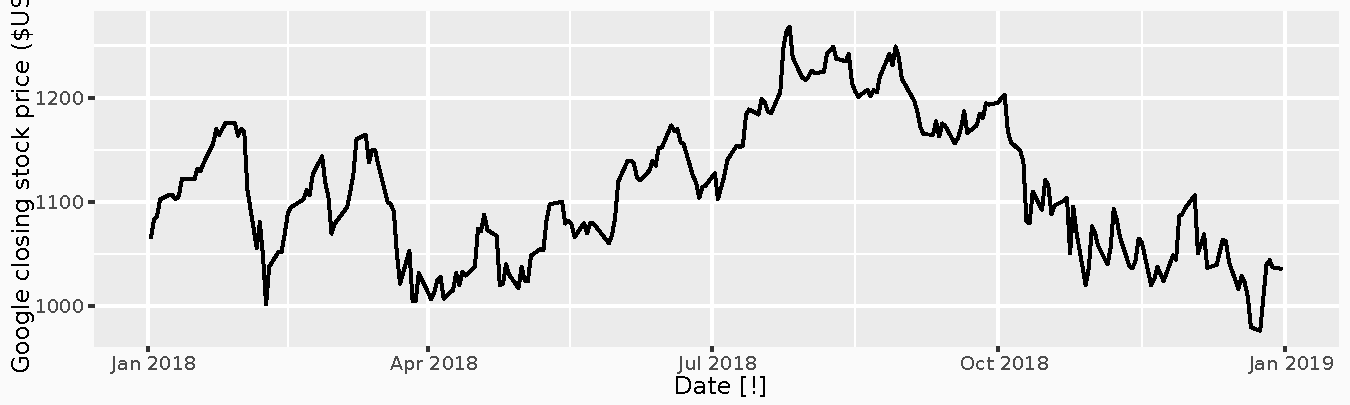
\includegraphics{04_arima_files/figure-beamer/unnamed-chunk-2-1.pdf}
\end{frame}

\begin{frame}[fragile]{Stationary?}
\protect\hypertarget{stationary-1}{}
\fontsize{11}{12}\sf

\begin{Shaded}
\begin{Highlighting}[]
\NormalTok{gafa\_stock }\SpecialCharTok{|\textgreater{}}
  \FunctionTok{filter}\NormalTok{(Symbol }\SpecialCharTok{==} \StringTok{"GOOG"}\NormalTok{, }\FunctionTok{year}\NormalTok{(Date) }\SpecialCharTok{==} \DecValTok{2018}\NormalTok{) }\SpecialCharTok{|\textgreater{}}
  \FunctionTok{autoplot}\NormalTok{(}\FunctionTok{difference}\NormalTok{(Close)) }\SpecialCharTok{+}
  \FunctionTok{labs}\NormalTok{(}\AttributeTok{y =} \StringTok{"Daily change in Google closing stock price"}\NormalTok{)}
\end{Highlighting}
\end{Shaded}

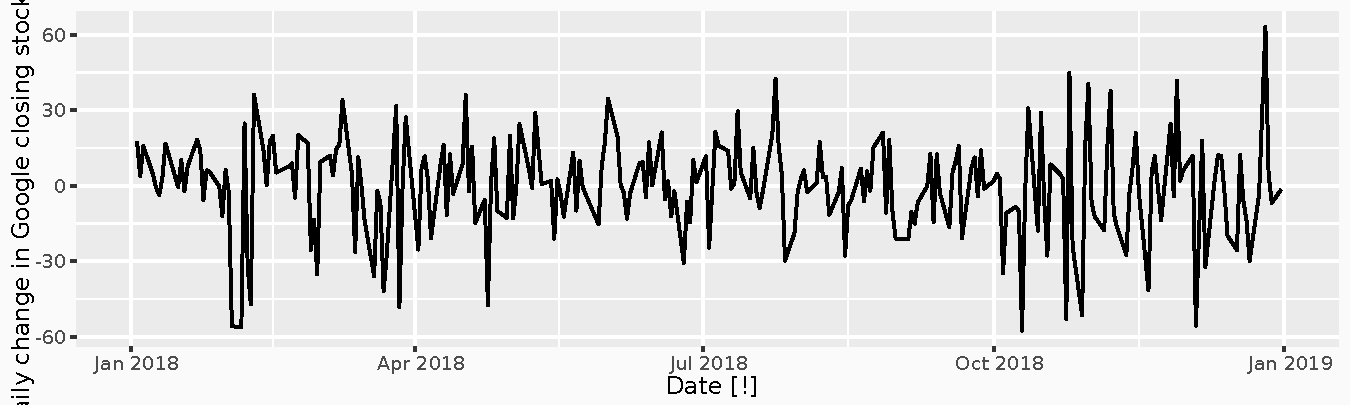
\includegraphics{04_arima_files/figure-beamer/unnamed-chunk-3-1.pdf}
\end{frame}

\begin{frame}{Differencing}
\protect\hypertarget{differencing}{}
\fontsize{13}{15}\sf

\begin{itemize}
\tightlist
\item
  Differencing helps to \textbf{stabilize the mean}.
\item
  The differenced series is the \emph{change} between each observation
  in the original series.
\item
  Occasionally the differenced data will not appear stationary and it
  may be necessary to difference the data a second time.
\item
  In practice, it is almost never necessary to go beyond second-order
  differences.
\end{itemize}
\end{frame}

\begin{frame}{Autoregressive models}
\protect\hypertarget{autoregressive-models}{}
\begin{block}{Autoregressive (AR) models:}\vspace*{-0.3cm}
$$
  y_{t} = c + \phi_{1}y_{t - 1} + \phi_{2}y_{t - 2} + \cdots + \phi_{p}y_{t - p} + \varepsilon_{t},
$$
where $\varepsilon_t$ is white noise. A multiple regression with \textbf{lagged values} of $y_t$ as predictors.
\end{block}

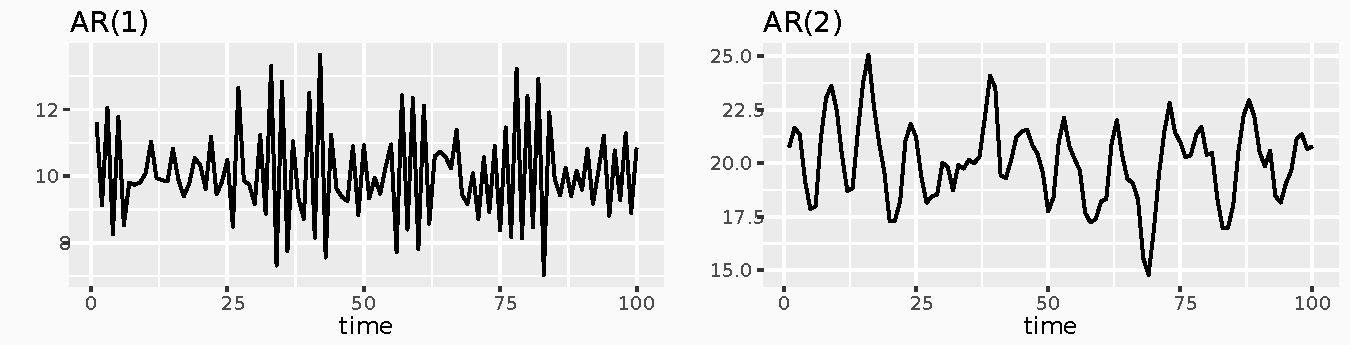
\includegraphics{04_arima_files/figure-beamer/arp-1.pdf}

\vspace*{-0.4cm}

\begin{itemize}
\tightlist
\item
  Cyclic behaviour is possible when \(p\ge 2\).
\end{itemize}
\end{frame}

\begin{frame}{Moving Average (MA) models}
\protect\hypertarget{moving-average-ma-models}{}
\begin{block}{Moving Average (MA) models:}\vspace*{-0.3cm}
$$
  y_{t} = c + \varepsilon_t + \theta_{1}\varepsilon_{t - 1} + \theta_{2}\varepsilon_{t - 2} + \cdots + \theta_{q}\varepsilon_{t - q},
$$
where $\varepsilon_t$ is white noise.
A multiple regression with \textbf{lagged \emph{errors}} as predictors. \emph{Don't confuse with moving average smoothing!}
\end{block}

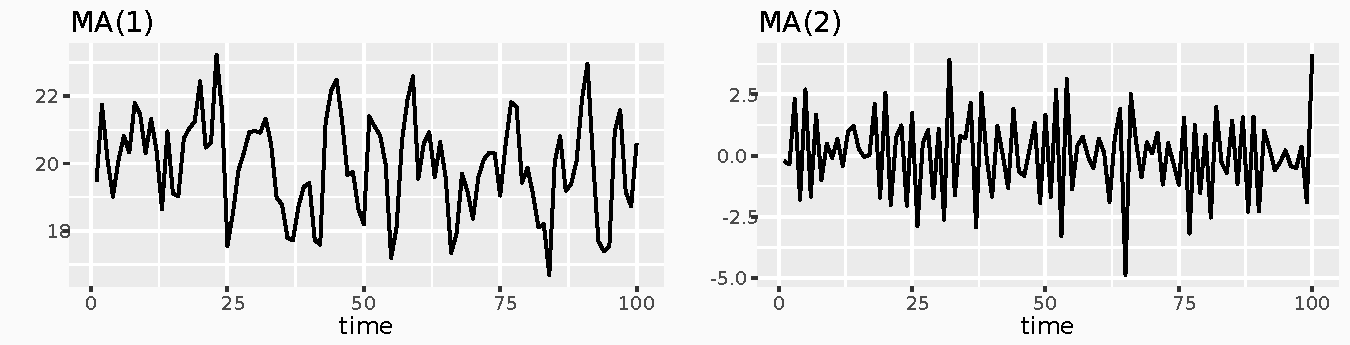
\includegraphics{04_arima_files/figure-beamer/maq-1.pdf}
\end{frame}

\begin{frame}{ARIMA models}
\protect\hypertarget{arima-models-2}{}
\begin{block}{Autoregressive Moving Average models:}\vspace*{-0.7cm}
\begin{align*}
  y_{t} &= c + \phi_{1}y_{t - 1} + \cdots + \phi_{p}y_{t - p} \\
        & \hspace*{2.4cm}\text{} + \theta_{1}\varepsilon_{t - 1} + \cdots + \theta_{q}\varepsilon_{t - q} + \varepsilon_{t}.
\end{align*}
\end{block}\pause

\begin{itemize}
\tightlist
\item
  Predictors include both \textbf{lagged values of \(y_t\) and lagged
  errors.} \pause
\end{itemize}

\begin{block}{Autoregressive Integrated Moving Average models}
\protect\hypertarget{autoregressive-integrated-moving-average-models}{}
\begin{itemize}
\tightlist
\item
  Combine ARMA model with \textbf{differencing}.
\item
  \(d\)-differenced series follows an ARMA model.
\item
  Need to choose \(p\), \(d\), \(q\) and whether or not to include
  \(c\).
\end{itemize}
\end{block}
\end{frame}

\begin{frame}{ARIMA models}
\protect\hypertarget{arima-models-3}{}
\begin{block}{ARIMA($p, d, q$) model}
\begin{tabular}{rl}
AR:& $p =$ order of the autoregressive part\\
I: & $d =$ degree of first differencing involved\\
MA:& $q =$ order of the moving average part.
\end{tabular}
\end{block}

\begin{itemize}
\tightlist
\item
  White noise model: ARIMA(0,0,0)
\item
  Random walk: ARIMA(0,1,0) with no constant
\item
  Random walk with drift: ARIMA(0,1,0) with \rlap{const.}
\item
  AR(\(p\)): ARIMA(\(p\),0,0)
\item
  MA(\(q\)): ARIMA(0,0,\(q\))
\end{itemize}
\end{frame}

\begin{frame}[fragile]{Example: National populations}
\protect\hypertarget{example-national-populations}{}
\fontsize{11}{12}\sf

\begin{Shaded}
\begin{Highlighting}[]
\NormalTok{fit }\OtherTok{\textless{}{-}}\NormalTok{ global\_economy }\SpecialCharTok{|\textgreater{}}
  \FunctionTok{model}\NormalTok{(}\AttributeTok{arima =} \FunctionTok{ARIMA}\NormalTok{(Population))}
\NormalTok{fit}
\end{Highlighting}
\end{Shaded}

\begin{verbatim}
# A mable: 263 x 2
# Key:     Country [263]
   Country                               arima
   <fct>                               <model>
 1 Afghanistan                  <ARIMA(4,2,1)>
 2 Albania                      <ARIMA(0,2,2)>
 3 Algeria                      <ARIMA(2,2,2)>
 4 American Samoa               <ARIMA(2,2,2)>
 5 Andorra             <ARIMA(2,1,2) w/ drift>
 6 Angola                       <ARIMA(4,2,1)>
 7 Antigua and Barbuda <ARIMA(2,1,2) w/ drift>
 8 Arab World                   <ARIMA(0,2,1)>
 9 Argentina                    <ARIMA(2,2,2)>
10 Armenia                      <ARIMA(3,2,0)>
# i 253 more rows
\end{verbatim}
\end{frame}

\begin{frame}[fragile]{Example: National populations}
\protect\hypertarget{example-national-populations-1}{}
\fontsize{11}{12}\sf

\begin{Shaded}
\begin{Highlighting}[]
\NormalTok{fit }\SpecialCharTok{|\textgreater{}}
  \FunctionTok{filter}\NormalTok{(Country }\SpecialCharTok{==} \StringTok{"Australia"}\NormalTok{) }\SpecialCharTok{|\textgreater{}}
  \FunctionTok{report}\NormalTok{()}
\end{Highlighting}
\end{Shaded}

\begin{verbatim}
Series: Population 
Model: ARIMA(0,2,1) 

Coefficients:
         ma1
      -0.661
s.e.   0.107

sigma^2 estimated as 4.063e+09:  log likelihood=-699
AIC=1401   AICc=1402   BIC=1405
\end{verbatim}

\only<2>{\begin{textblock}{6.4}(6,4.6)
\begin{alertblock}{}\fontsize{12}{13}\sf
\centerline{$y_t = 2y_{t-1} - y_{t-2} - 0.7 \varepsilon_{t-1} + \varepsilon_t$}
\mbox{}\hfill$\varepsilon_t \sim \text{NID}(0,4\times10^9)$
\end{alertblock}
\end{textblock}}
\vspace*{3cm}
\end{frame}

\begin{frame}{Understanding ARIMA models}
\protect\hypertarget{understanding-arima-models}{}
\begin{itemize}
\tightlist
\item
  If \(c=0\) and \(d=0\), the long-term forecasts will go to zero.
\item
  If \(c=0\) and \(d=1\), the long-term forecasts will go to a non-zero
  constant.
\item
  If \(c=0\) and \(d=2\), the long-term forecasts will follow a straight
  line.
\item
  If \(c\ne0\) and \(d=0\), the long-term forecasts will go to the mean
  of the data.
\item
  If \(c\ne0\) and \(d=1\), the long-term forecasts will follow a
  straight line.
\item
  If \(c\ne0\) and \(d=2\), the long-term forecasts will follow a
  quadratic trend.
\end{itemize}
\end{frame}

\begin{frame}{Understanding ARIMA models}
\protect\hypertarget{understanding-arima-models-1}{}
\fontsize{14}{15.5}\sf

\begin{block}{Forecast variance and \(d\)}
\protect\hypertarget{forecast-variance-and-d}{}
\begin{itemize}
\tightlist
\item
  The higher the value of \(d\), the more rapidly the prediction
  intervals increase in size.
\item
  For \(d=0\), the long-term forecast standard deviation will go to the
  standard deviation of the historical data.
\end{itemize}
\end{block}
\end{frame}

\begin{frame}[fragile]{Example: National populations}
\protect\hypertarget{example-national-populations-2}{}
\fontsize{9}{9}\sf

\begin{Shaded}
\begin{Highlighting}[]
\NormalTok{fit }\SpecialCharTok{|\textgreater{}}
  \FunctionTok{forecast}\NormalTok{(}\AttributeTok{h =} \DecValTok{10}\NormalTok{) }\SpecialCharTok{|\textgreater{}}
  \FunctionTok{filter}\NormalTok{(Country }\SpecialCharTok{==} \StringTok{"Australia"}\NormalTok{) }\SpecialCharTok{|\textgreater{}}
  \FunctionTok{autoplot}\NormalTok{(global\_economy)}
\end{Highlighting}
\end{Shaded}

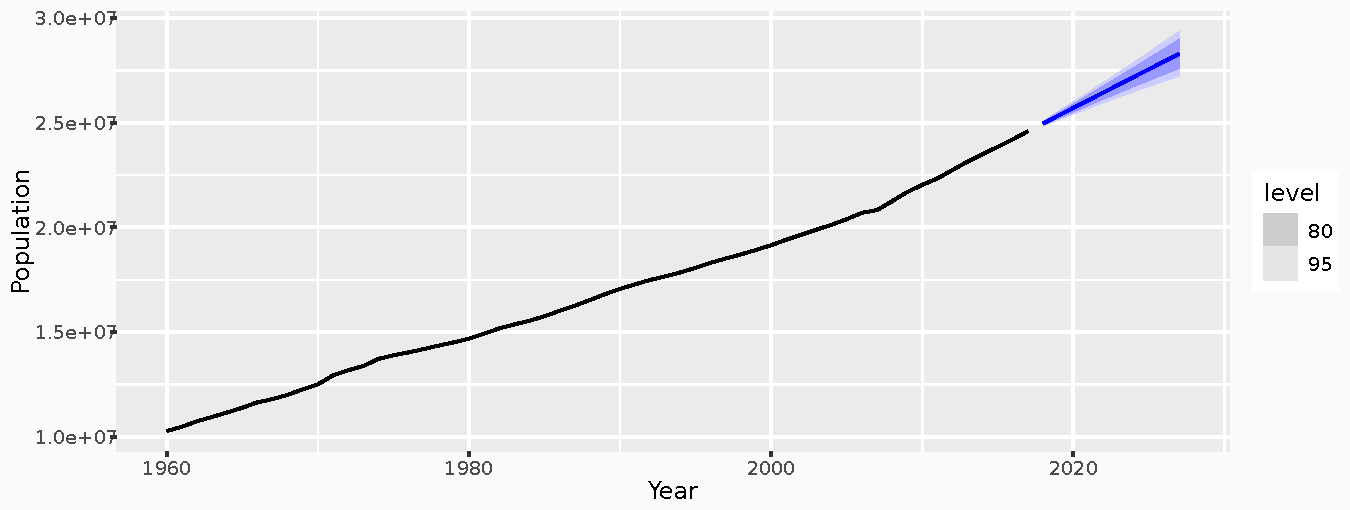
\includegraphics{04_arima_files/figure-beamer/popfc2-1.pdf}
\end{frame}

\begin{frame}{How does ARIMA() work?}
\protect\hypertarget{how-does-arima-work}{}
\begin{alertblock}{Hyndman and Khandakar (JSS, 2008) algorithm:}
\begin{itemize}\tightlist
\item Select no.\ differences $d$ via KPSS test.
\item Select $p$, $q$ and inclusion of $c$ by minimising AICc.
\item Use stepwise search to traverse model space.
\end{itemize}
\end{alertblock}\pause

\begin{block}{}
\centerline{$\displaystyle \text{AICc} = -2 \log(L) + 2(p+q+k+1)\left[1 + \frac{(p+q+k+2)}{T-p-q-k-2}\right]$}
where $L$ is the maximised likelihood fitted to the \textit{differenced} data,
$k=1$ if $c\neq 0$ and $k=0$ otherwise.\pause
\end{block}

Note: Can't compare AICc for different values of \(d\).
\end{frame}

\begin{frame}{How does ARIMA() work?}
\protect\hypertarget{how-does-arima-work-1}{}
\fontsize{12.5}{14.5}\sf

\begin{description}
\item[Step1:]
Select current model (with smallest AICc) from:\newline
ARIMA\((2,d,2)\)\newline ARIMA\((0,d,0)\)\newline
ARIMA\((1,d,0)\)\newline ARIMA\((0,d,1)\) \pause\vspace*{-0.1cm}
\item[Step 2:]
Consider variations of current model:

\begin{itemize}
\tightlist
\item
  vary one of \(p,q,\) from current model by \(\pm1\);
\item
  \(p,q\) both vary from current model by \(\pm1\);
\item
  Include/exclude \(c\) from current model.
\end{itemize}
\end{description}

Model with lowest AICc becomes current model.

\pause\alert{Repeat Step 2 until no lower AICc can be found.}
\end{frame}

\begin{frame}{How does ARIMA() work?}
\protect\hypertarget{how-does-arima-work-2}{}
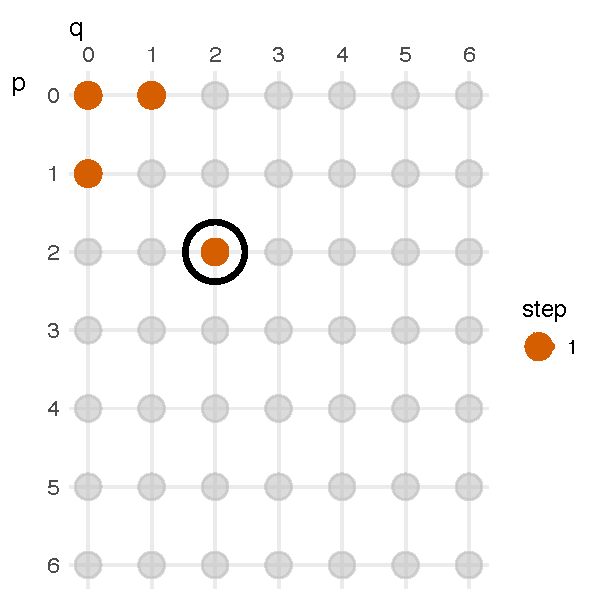
\includegraphics[width=0.6\textwidth,height=\textheight]{04_arima_files/figure-beamer/ARMAgridsearch-1.pdf}
\end{frame}

\begin{frame}{How does ARIMA() work?}
\protect\hypertarget{how-does-arima-work-3}{}
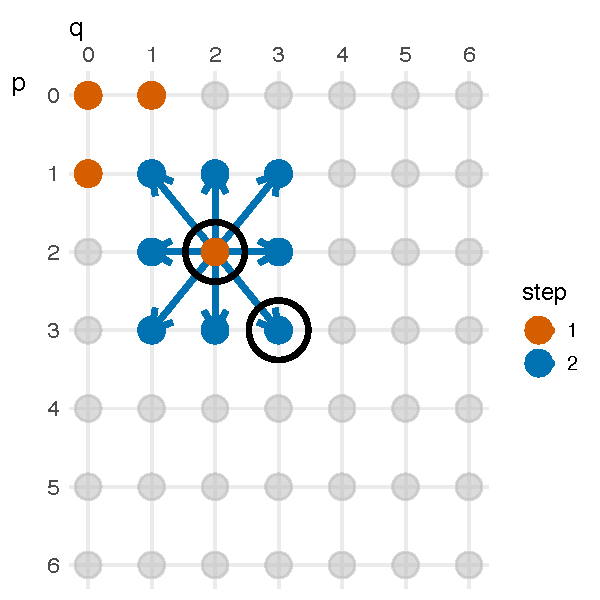
\includegraphics[width=0.6\textwidth,height=\textheight]{04_arima_files/figure-beamer/ARMAgridsearch2-1.pdf}
\end{frame}

\begin{frame}{How does ARIMA() work?}
\protect\hypertarget{how-does-arima-work-4}{}
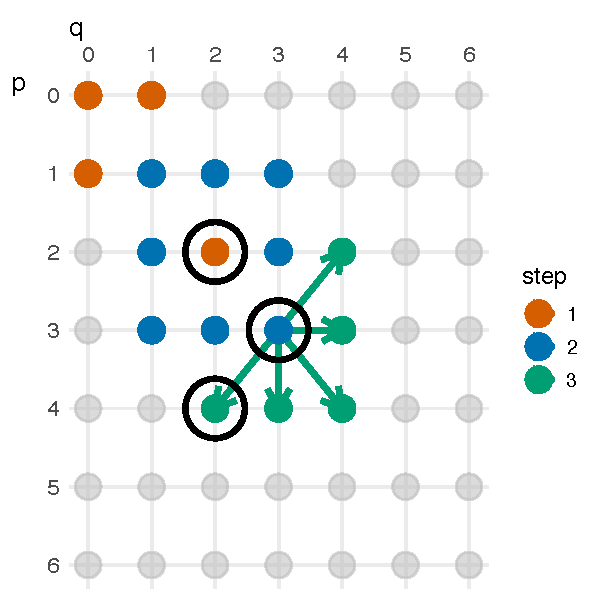
\includegraphics[width=0.6\textwidth,height=\textheight]{04_arima_files/figure-beamer/ARMAgridsearch3-1.pdf}
\end{frame}

\begin{frame}{How does ARIMA() work?}
\protect\hypertarget{how-does-arima-work-5}{}
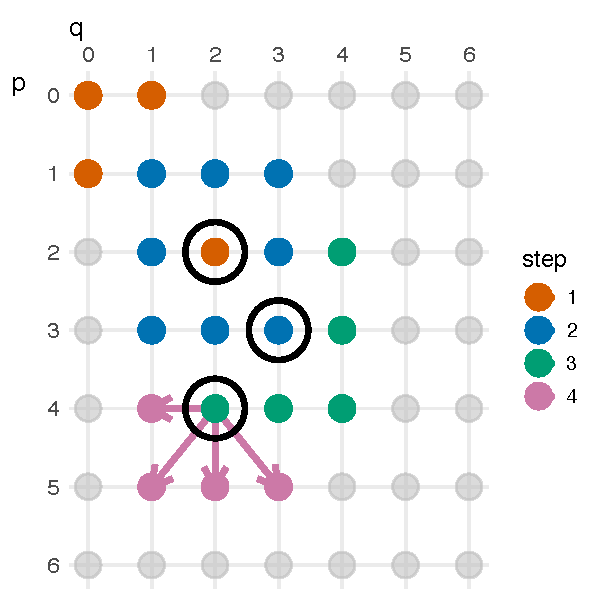
\includegraphics[width=0.6\textwidth,height=\textheight]{04_arima_files/figure-beamer/ARMAgridsearch4-1.pdf}
\end{frame}

\hypertarget{seasonal-arima-models}{%
\section{Seasonal ARIMA models}\label{seasonal-arima-models}}

\begin{frame}{Seasonal ARIMA models}
\protect\hypertarget{seasonal-arima-models-1}{}
\fontsize{13}{15}\sf

\begin{longtable}[]{@{}rcc@{}}
\toprule\noalign{}
ARIMA & \(~\underbrace{(p, d, q)}\) & \(\underbrace{(P, D, Q)_{m}}\) \\
\midrule\noalign{}
\endhead
& \({\uparrow}\) & \({\uparrow}\) \\
& Non-seasonal part & Seasonal part of \\
& of the model & of the model \\
\bottomrule\noalign{}
\end{longtable}

\vspace*{-0.4cm}

\begin{itemize}
\tightlist
\item
  \(m =\) number of observations per year.
\item
  \(d\) first differences, \(D\) seasonal differences
\item
  \(p\) AR lags, \(q\) MA lags
\item
  \(P\) seasonal AR lags, \(Q\) seasonal MA lags
\end{itemize}

\begin{block}{}
\protect\hypertarget{section-1}{}
Seasonal and non-seasonal terms combine multiplicatively
\end{block}
\end{frame}

\begin{frame}[fragile]{Cortecosteroid drug sales}
\protect\hypertarget{cortecosteroid-drug-sales}{}
\begin{Shaded}
\begin{Highlighting}[]
\NormalTok{h02 }\OtherTok{\textless{}{-}}\NormalTok{ PBS }\SpecialCharTok{|\textgreater{}}
  \FunctionTok{filter}\NormalTok{(ATC2 }\SpecialCharTok{==} \StringTok{"H02"}\NormalTok{) }\SpecialCharTok{|\textgreater{}}
  \FunctionTok{summarise}\NormalTok{(}\AttributeTok{Cost =} \FunctionTok{sum}\NormalTok{(Cost) }\SpecialCharTok{/} \FloatTok{1e6}\NormalTok{)}
\end{Highlighting}
\end{Shaded}
\end{frame}

\begin{frame}[fragile]{Cortecosteroid drug sales}
\protect\hypertarget{cortecosteroid-drug-sales-1}{}
\begin{Shaded}
\begin{Highlighting}[]
\NormalTok{h02 }\SpecialCharTok{|\textgreater{}} \FunctionTok{autoplot}\NormalTok{(}
\NormalTok{  Cost}
\NormalTok{)}
\end{Highlighting}
\end{Shaded}

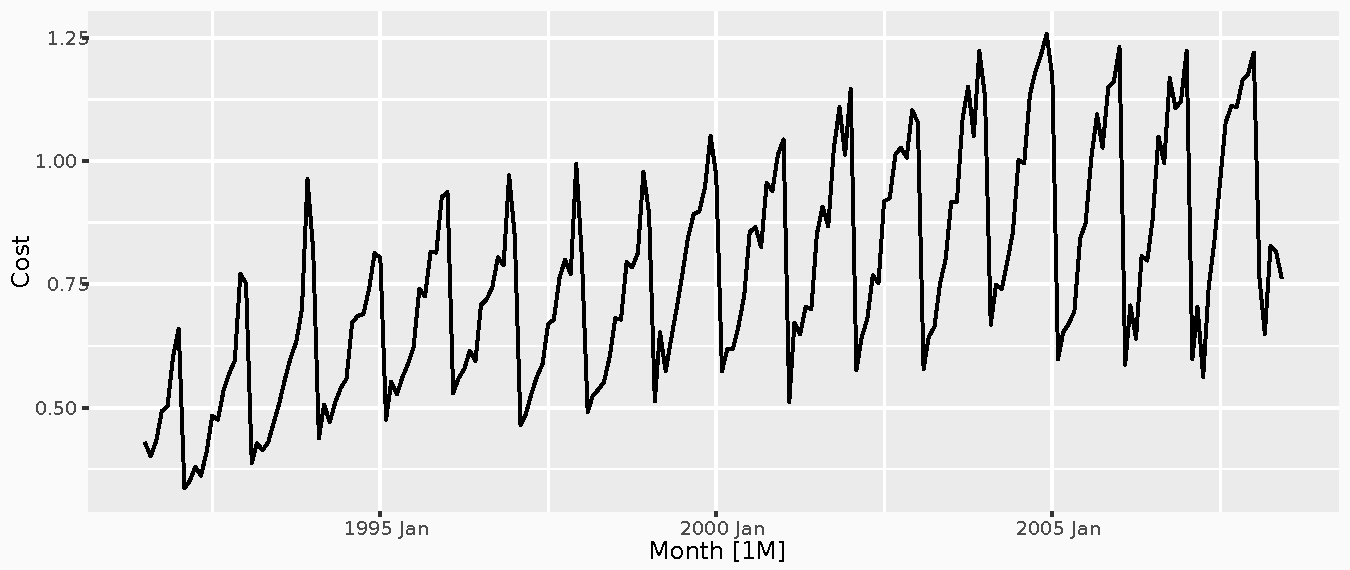
\includegraphics{04_arima_files/figure-beamer/unnamed-chunk-5-1.pdf}
\end{frame}

\begin{frame}[fragile]{Cortecosteroid drug sales}
\protect\hypertarget{cortecosteroid-drug-sales-2}{}
\begin{Shaded}
\begin{Highlighting}[]
\NormalTok{h02 }\SpecialCharTok{|\textgreater{}} \FunctionTok{autoplot}\NormalTok{(}
  \FunctionTok{log}\NormalTok{(Cost)}
\NormalTok{)}
\end{Highlighting}
\end{Shaded}

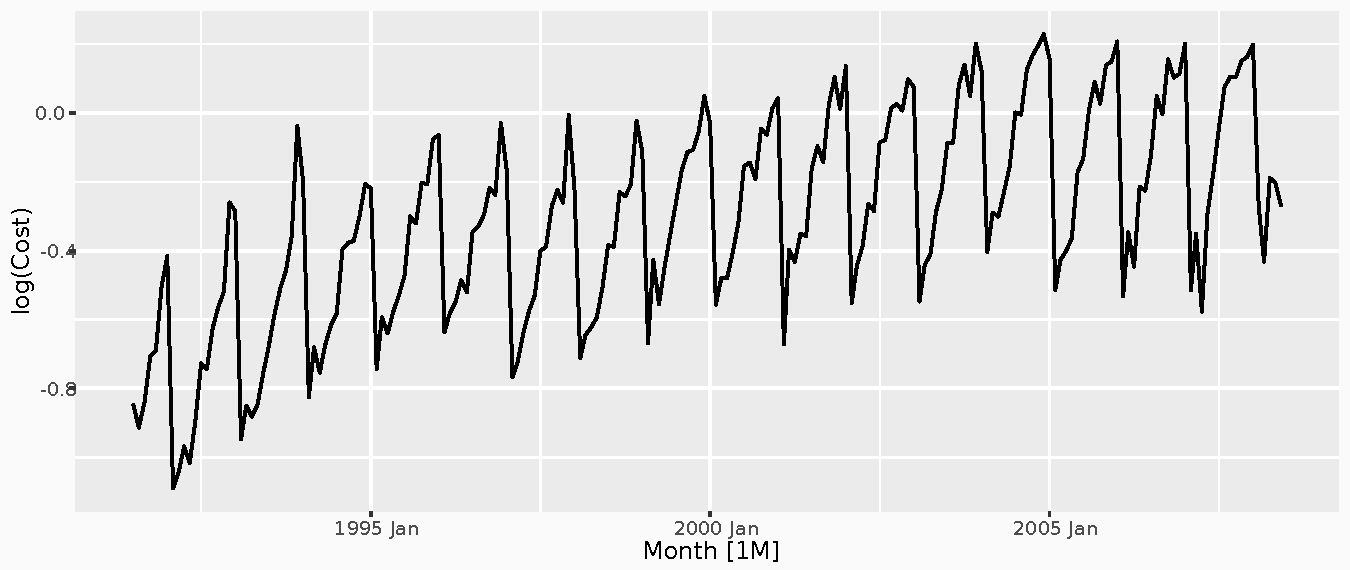
\includegraphics{04_arima_files/figure-beamer/unnamed-chunk-6-1.pdf}
\end{frame}

\begin{frame}[fragile]{Cortecosteroid drug sales}
\protect\hypertarget{cortecosteroid-drug-sales-3}{}
\begin{Shaded}
\begin{Highlighting}[]
\NormalTok{h02 }\SpecialCharTok{|\textgreater{}} \FunctionTok{autoplot}\NormalTok{(}
  \FunctionTok{log}\NormalTok{(Cost) }\SpecialCharTok{|\textgreater{}} \FunctionTok{difference}\NormalTok{(}\DecValTok{12}\NormalTok{)}
\NormalTok{)}
\end{Highlighting}
\end{Shaded}

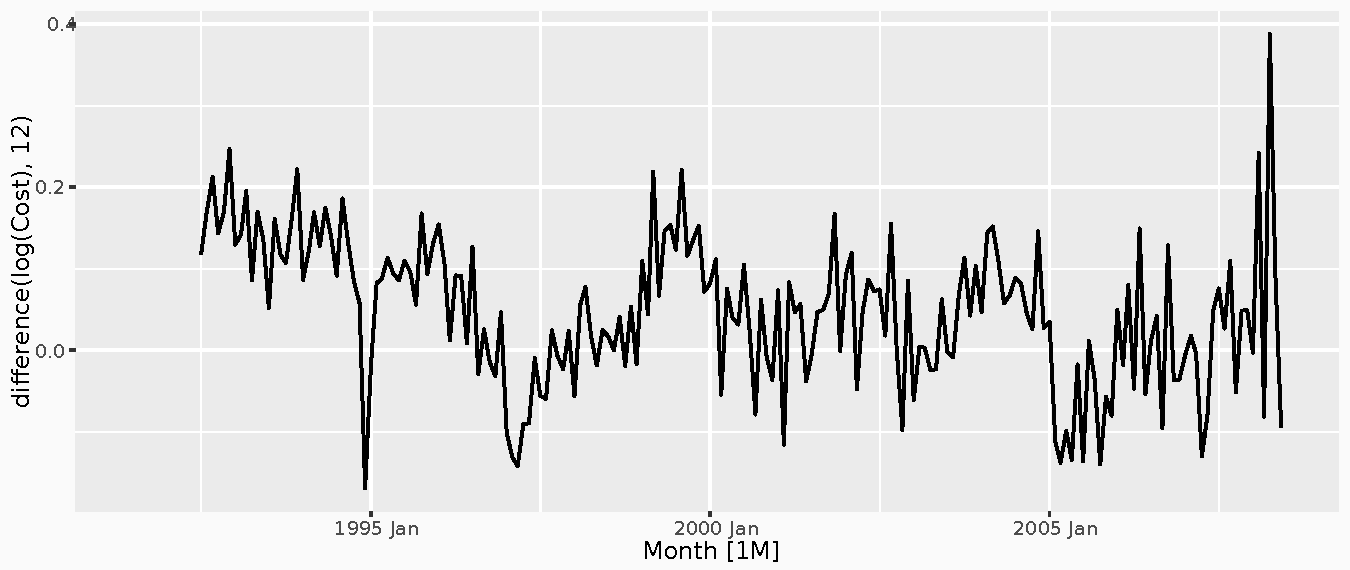
\includegraphics{04_arima_files/figure-beamer/unnamed-chunk-7-1.pdf}
\end{frame}

\begin{frame}[fragile]{Cortecosteroid drug sales}
\protect\hypertarget{cortecosteroid-drug-sales-4}{}
\begin{Shaded}
\begin{Highlighting}[]
\NormalTok{h02 }\SpecialCharTok{|\textgreater{}} \FunctionTok{autoplot}\NormalTok{(}
  \FunctionTok{log}\NormalTok{(Cost) }\SpecialCharTok{|\textgreater{}} \FunctionTok{difference}\NormalTok{(}\DecValTok{12}\NormalTok{) }\SpecialCharTok{|\textgreater{}} \FunctionTok{difference}\NormalTok{(}\DecValTok{1}\NormalTok{)}
\NormalTok{)}
\end{Highlighting}
\end{Shaded}

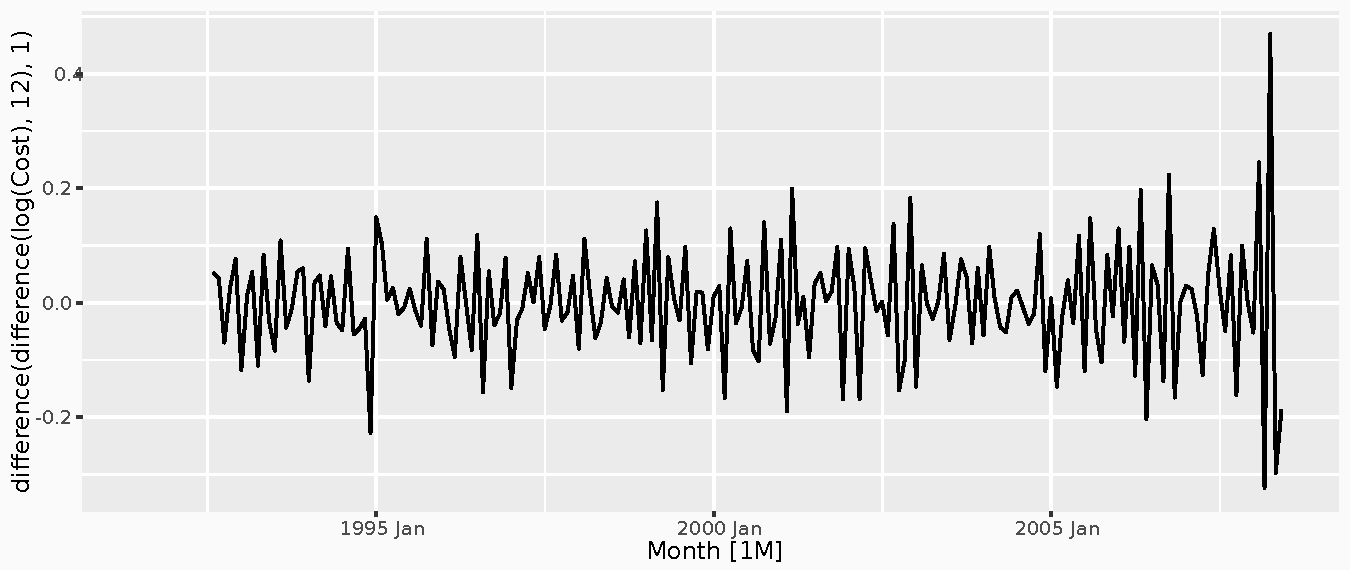
\includegraphics{04_arima_files/figure-beamer/unnamed-chunk-8-1.pdf}
\end{frame}

\begin{frame}[fragile]{Cortecosteroid drug sales}
\protect\hypertarget{cortecosteroid-drug-sales-5}{}
\fontsize{11}{12}\sf

\begin{Shaded}
\begin{Highlighting}[]
\NormalTok{h02 }\SpecialCharTok{|\textgreater{}}
  \FunctionTok{model}\NormalTok{(}\AttributeTok{arima =} \FunctionTok{ARIMA}\NormalTok{(}\FunctionTok{log}\NormalTok{(Cost))) }\SpecialCharTok{|\textgreater{}}
  \FunctionTok{report}\NormalTok{()}
\end{Highlighting}
\end{Shaded}

\begin{verbatim}
Series: Cost 
Model: ARIMA(2,1,0)(0,1,1)[12] 
Transformation: log(Cost) 

Coefficients:
          ar1      ar2     sma1
      -0.8491  -0.4207  -0.6401
s.e.   0.0712   0.0714   0.0694

sigma^2 estimated as 0.004387:  log likelihood=245
AIC=-483   AICc=-483   BIC=-470
\end{verbatim}
\end{frame}

\begin{frame}[fragile]{Cortecosteroid drug sales}
\protect\hypertarget{cortecosteroid-drug-sales-6}{}
\fontsize{11}{13}\sf

\begin{Shaded}
\begin{Highlighting}[]
\NormalTok{h02 }\SpecialCharTok{|\textgreater{}}
  \FunctionTok{model}\NormalTok{(}\AttributeTok{arima =} \FunctionTok{ARIMA}\NormalTok{(}\FunctionTok{log}\NormalTok{(Cost))) }\SpecialCharTok{|\textgreater{}}
  \FunctionTok{forecast}\NormalTok{(}\AttributeTok{h =} \StringTok{"3 years"}\NormalTok{) }\SpecialCharTok{|\textgreater{}}
  \FunctionTok{autoplot}\NormalTok{(h02)}
\end{Highlighting}
\end{Shaded}

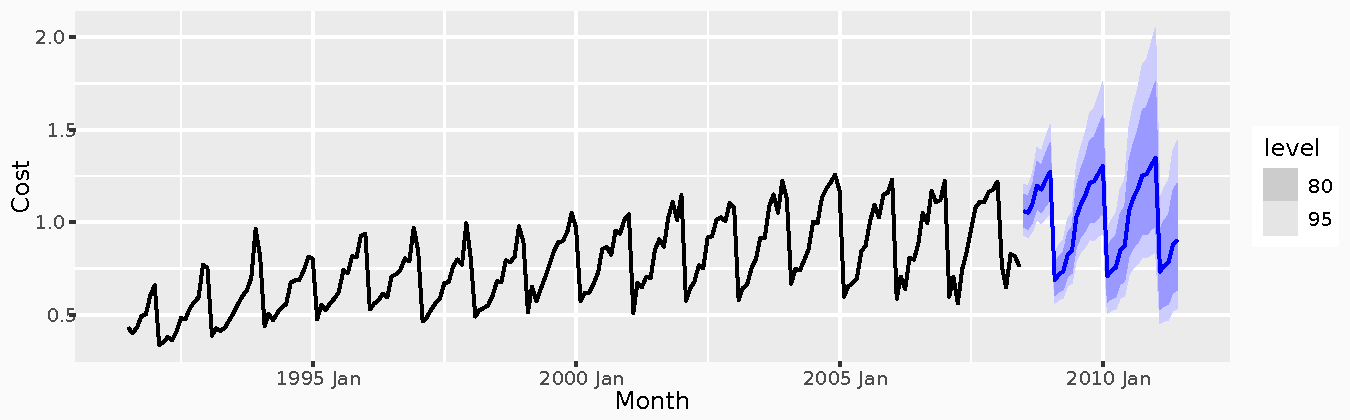
\includegraphics{04_arima_files/figure-beamer/h02fcst-1.pdf}

\vspace*{5cm}
\end{frame}

\begin{frame}[fragile]{Cortecosteroid drug sales}
\protect\hypertarget{cortecosteroid-drug-sales-7}{}
\fontsize{9}{9}\sf

\begin{Shaded}
\begin{Highlighting}[]
\NormalTok{fit }\OtherTok{\textless{}{-}}\NormalTok{ h02 }\SpecialCharTok{|\textgreater{}}
  \FunctionTok{model}\NormalTok{(}\AttributeTok{best =} \FunctionTok{ARIMA}\NormalTok{(}\FunctionTok{log}\NormalTok{(Cost),}
    \AttributeTok{stepwise =} \ConstantTok{FALSE}\NormalTok{,}
    \AttributeTok{approximation =} \ConstantTok{FALSE}\NormalTok{,}
    \AttributeTok{order\_constraint =}\NormalTok{ p }\SpecialCharTok{+}\NormalTok{ q }\SpecialCharTok{+}\NormalTok{ P }\SpecialCharTok{+}\NormalTok{ Q }\SpecialCharTok{\textless{}=} \DecValTok{9}
\NormalTok{  ))}
\FunctionTok{report}\NormalTok{(fit)}
\end{Highlighting}
\end{Shaded}

\begin{verbatim}
Series: Cost 
Model: ARIMA(4,1,1)(2,1,2)[12] 
Transformation: log(Cost) 

Coefficients:
          ar1    ar2    ar3     ar4     ma1   sar1    sar2    sma1   sma2
      -0.0425  0.210  0.202  -0.227  -0.742  0.621  -0.383  -1.202  0.496
s.e.   0.2167  0.181  0.114   0.081   0.207  0.242   0.118   0.249  0.213

sigma^2 estimated as 0.004049:  log likelihood=254
AIC=-489   AICc=-487   BIC=-456
\end{verbatim}
\end{frame}

\begin{frame}[fragile]{Cortecosteroid drug sales}
\protect\hypertarget{cortecosteroid-drug-sales-8}{}
\fontsize{11}{14}\sf

\begin{Shaded}
\begin{Highlighting}[]
\NormalTok{fit }\SpecialCharTok{|\textgreater{}}
  \FunctionTok{forecast}\NormalTok{() }\SpecialCharTok{|\textgreater{}}
  \FunctionTok{autoplot}\NormalTok{(h02) }\SpecialCharTok{+}
  \FunctionTok{labs}\NormalTok{(}\AttributeTok{y =} \StringTok{"H02 Expenditure ($AUD)"}\NormalTok{, }\AttributeTok{x =} \StringTok{"Year"}\NormalTok{)}
\end{Highlighting}
\end{Shaded}

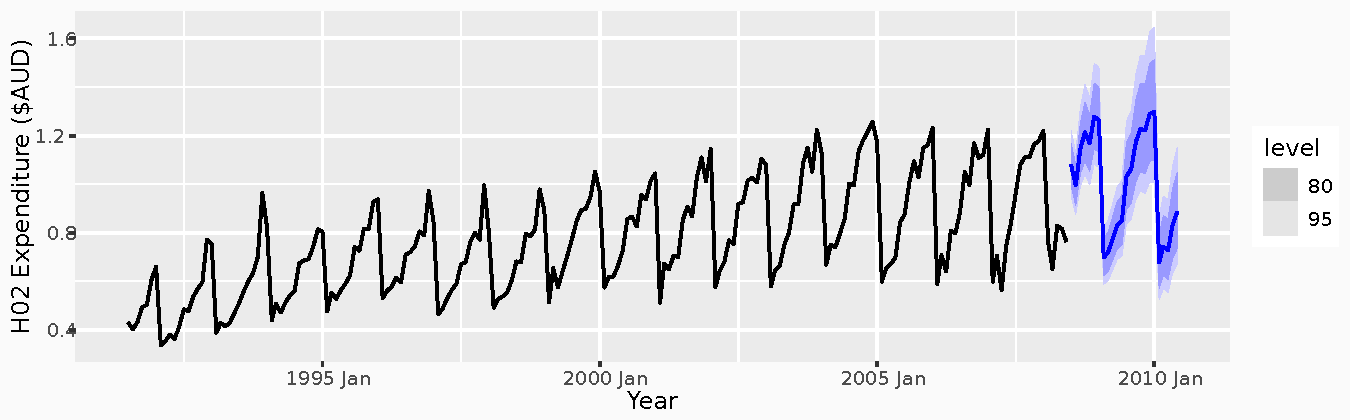
\includegraphics{04_arima_files/figure-beamer/h02f-1.pdf}
\end{frame}

\hypertarget{forecast-ensembles}{%
\section{Forecast ensembles}\label{forecast-ensembles}}

\begin{frame}[fragile]{Forecast ensembles}
\protect\hypertarget{forecast-ensembles-1}{}
\fontsize{10}{11}\sf

\begin{Shaded}
\begin{Highlighting}[]
\NormalTok{train }\OtherTok{\textless{}{-}}\NormalTok{ tourism }\SpecialCharTok{|\textgreater{}}
  \FunctionTok{filter}\NormalTok{(}\FunctionTok{year}\NormalTok{(Quarter) }\SpecialCharTok{\textless{}=} \DecValTok{2014}\NormalTok{)}
\NormalTok{fit }\OtherTok{\textless{}{-}}\NormalTok{ train }\SpecialCharTok{|\textgreater{}}
  \FunctionTok{model}\NormalTok{(}
    \AttributeTok{ets =} \FunctionTok{ETS}\NormalTok{(Trips),}
    \AttributeTok{arima =} \FunctionTok{ARIMA}\NormalTok{(Trips),}
    \AttributeTok{snaive =} \FunctionTok{SNAIVE}\NormalTok{(Trips)}
\NormalTok{  ) }\SpecialCharTok{|\textgreater{}}
  \FunctionTok{mutate}\NormalTok{(}\AttributeTok{mixed =}\NormalTok{ (ets }\SpecialCharTok{+}\NormalTok{ arima }\SpecialCharTok{+}\NormalTok{ snaive) }\SpecialCharTok{/} \DecValTok{3}\NormalTok{)}
\end{Highlighting}
\end{Shaded}

\fontsize{13}{14}\sf

\begin{itemize}
\tightlist
\item
  Ensemble forecast \texttt{mixed} is a simple average of the three
  fitted models.
\item
  \texttt{forecast()} will produce distributional forecasts taking into
  account the correlations between the forecast errors of the component
  models.
\end{itemize}
\end{frame}

\begin{frame}[fragile]{Forecast ensembles}
\protect\hypertarget{forecast-ensembles-2}{}
\fontsize{10}{11}\sf

\begin{Shaded}
\begin{Highlighting}[]
\NormalTok{fc }\OtherTok{\textless{}{-}}\NormalTok{ fit }\SpecialCharTok{|\textgreater{}} \FunctionTok{forecast}\NormalTok{(}\AttributeTok{h =} \StringTok{"3 years"}\NormalTok{)}
\NormalTok{fc }\SpecialCharTok{|\textgreater{}}
  \FunctionTok{filter}\NormalTok{(Region }\SpecialCharTok{==} \StringTok{"Snowy Mountains"}\NormalTok{, Purpose }\SpecialCharTok{==} \StringTok{"Holiday"}\NormalTok{) }\SpecialCharTok{|\textgreater{}}
  \FunctionTok{autoplot}\NormalTok{(tourism, }\AttributeTok{level =} \ConstantTok{NULL}\NormalTok{)}
\end{Highlighting}
\end{Shaded}

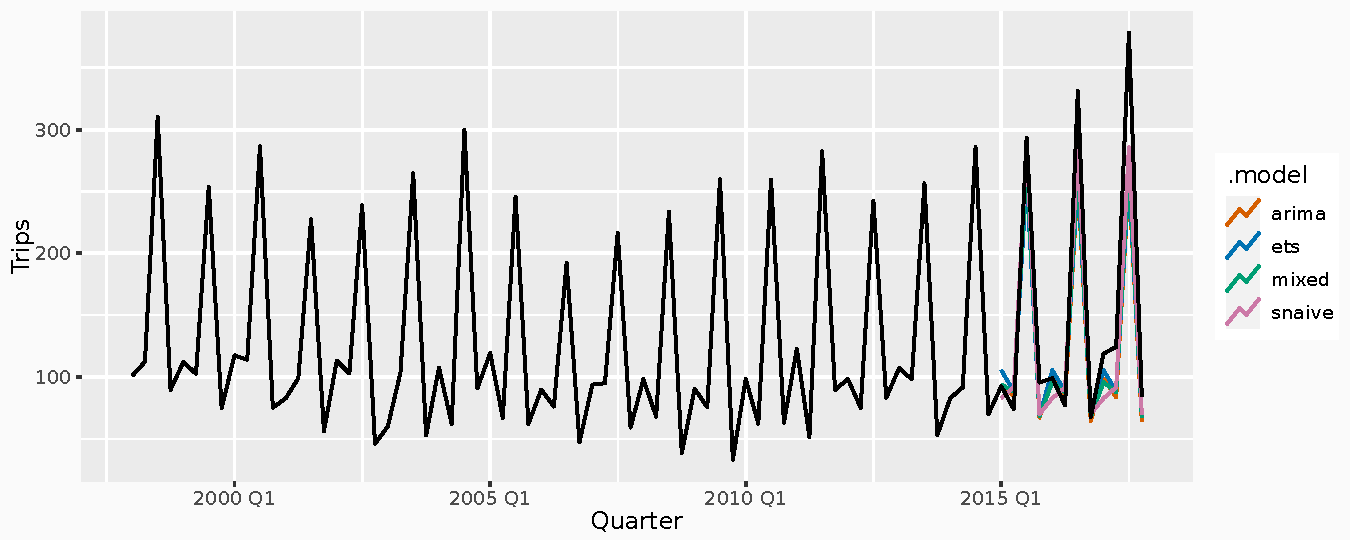
\includegraphics{04_arima_files/figure-beamer/trainfc-1.pdf}
\end{frame}



\end{document}
